\documentclass[../../index.tex]{subfiles}

\begin{document}
  \chapter{Derivation of the used inverse covariance matrix from the Aleph
    data}
  While performing a \textbf{Generalized least squares} (GLS) we estimate our
  regression coefficients $\hat\beta$ as follows:
  \begin{equation}
    \hat\beta = \underset{b}{\operatorname {argmin}}(\mathbf{y} - \mathbf{X} \mathbf{b}
    )^{\mathtt{T}} \mathbf{\Omega}^{-1} (\mathbf{y} - \mathbf{X} \mathbf{b}),
  \end{equation}
  with $\mathbf{b}$ being an candidate estimate of $\beta$, $\mathbf{X}$ being the
  design matrix, $\mathbf{y}$ being the response values and
  $\mathbf{\Omega}^{-1}$ being the \textbf{inverse covariance matrix}.

  The Aleph data includes the \textbf{standard error} (SE), which
  are equal to the \textbf{standard deviation} as per definition. Furthermore
  Aleph provides the \textbf{correlation coefficients} of the errors. We will
  use these two quantities in combination with \textbf{Gaussian error
    propagation} to derive derive an approximation of the covariance matrix.

  \section{Propagation of experimental errors and correlation}
  Let $\{f_k(x_1, x_2, \cdots x_n)\}$ be a set of $m$ functions, which a linear
  combinations of n variables $x_1, x_2, \cdots x_n$ with combination
  coefficients $A_{k1}, A_{k2}, \cdots A_{kn}$, where $k \in \{1, 2, \cdots,
  m\}$. Let the covariance matrix of $x_n$ be denoted by
  \begin{equation}
    \Sigma^x =
    \begin{pmatrix}
      \sigma_{1}^2 & \sigma_{12}  & \sigma_{13}  & \cdots \\
      \sigma_{12}  & \sigma_{2}^2 & \sigma_{23}  & \cdots \\
      \sigma_{13}  & \sigma_{23}  & \sigma_{3}^2 & \cdots \\
      \vdots      & \vdots       & \vdots      &  \ddots
    \end{pmatrix}.
  \end{equation}
  Then the covariance matrix of the functions $\Sigma^f$ is given by
  \begin{equation}
    \Sigma_{ij}^f = \sum_k^n \sum_l^n A_{ik} \sum_{kl}^x A_{jl}, \quad \Sigma^f= A \Sigma^x A^{\mathtt{T}}.
  \end{equation}

  In our case we are dealing with non-linear functions, which we will
  linearized with the help of the \textbf{Taylor expansion}
  \begin{equation}
    f_k \approx f_k^0 + \sum_i^n \frac{\partial f_k}{\partial x_i} x_i, \quad f \approx f^0 + Jx.
  \end{equation}
  Therefore, the propagation of error follows from the linear case, replacing
  the Jacobian matrix with the combination coefficients ($J = A$)
  % \begin{equation}
  %   \Sigma^f = J \Sigma^x J^{\mathtt{T}}.

  \chapter{Coefficients}
  \label{app:coefficients}
  \section{$\beta$ function}
  \label{sec:betaCoefficients}
  There are several conventions for defining the $\beta$ coefficients, depending
  on a minus sign and/or a factor of two (if one substitues $\mu \to \mu^2$) in
  the $\beta$-function \ref{eq:betaFunction}. We follow the convention from
  Pascual and Tarrach (except for the minus sign) and have taken the values from
  \cite{Boito2011}
  \begin{align}
    \beta_1 &= \frac{1}{6} (11N_c - 2N_f), \\
    \beta_2 &= \frac{1}{12} (17N_c^2 - 5N_cN_f - 3 C_fN_f), \\
    \beta_3 &= \frac{1}{32}\left( \frac{2857}{54}N_c^3 -\frac{1415}{54}N_c^2 N_f + \frac{79}{54} N_c N_f^2 - \frac{205}{18} N_c C_f N_f + \frac{11}{9} C_f N_f^2 + C_f^2 N_f \right), \\
    \beta_4 &= \frac{140599}{2304} + \frac{445}{16}\zeta_3,
  \end{align}
  where we used $N_f=3$ and $N_c=3$ for $\beta_4$.

  \section{Anomalous mass dimension}
  \label{app:gammaCoefficients}
  \begin{align}
    \gamma_1 &= \frac{3}{2}C_f, \\
    \gamma_2 &= \frac{C_f}{48}(97 N_c + 9 C_f - 10N_f), \\
    \gamma_3 &= \frac{C_f}{32}\left[ \frac{11413}{108} N_c^2 - \frac{129}{4} N_cC_f - \left( \frac{278}{27} + 24 \zeta_3 \right) N_c N_f + \frac{129}{2} C_f^2 - (23 - 24 \zeta_3) C_f N_f - \frac{35}{27} N_f^2 \right], \\
    \gamma_4 &= \frac{2977517}{20736} - \frac{9295}{216}\zeta_3 + \frac{135}{8}\zeta_4 - \frac{125}{6}\zeta_5,
  \end{align}
  where $N_c$ is the number of colours, $N_f$ the number of flavours and
  $C_f=(N_c^2-1)/2N_c$. We fixed furthermore fixed
  $N_f=3$ and $N_c=3$ for $\gamma_4$.


  \section{Adler function}

  \chapter{Källén-Lehmann spectral representation}
  \label{ch:kallenLehmannSpectralRepresentation}
In the second quantisation we applied latter operators $a_o^\dagger$ on the free
vacuum $\vert 0 \rangle$ to obtain single particle states, carrying a momentum
$p$
\begin{equation}
  a_p^\dagger \vert 0 \rangle = \frac{1}{\sqrt{2 E_p}}\vert \vec p \rangle,
\end{equation}
where the factor $\sqrt{2 E_p}$ is a convention resulting from the harmonic
oscillator. The identity operator for one\-/particle state, which selects only
single particle states is then given by
\begin{equation}
  \mathbb{1} = \int \frac{\dif^3 p}{(2\pi)^3} \frac{1}{2\omega_p} \vert \vec p \rangle \langle \vec p \vert.
\end{equation}
The above complete set of one\-/particle states can be enhanced to include
multiple\-/particle states, where we have to sum not only over all possible
momentum states $\vert \vec p \rangle$, but over all possible multi\-/particle
states and their enhanced states as well. If we define these state vectors as
$\vec X$ we can express the complete set of one\-/ and multiple\-/particle
states as
\begin{equation}
  \mathbb{1} = \intsum_{X} \dif \prod_X \vert X \rangle \langle  X \vert,
\end{equation}
where we have to sum over all possible $\vert X \rangle$ single- or
multi\-/particle states and integrate over the momentum $\vec p$ via
\begin{equation}
  \dif \Pi_X \equiv \prod_{i \in X} \int \frac{\dif^3 p_i}{(2\pi)^3} \frac{1}{2 E_j}.
\end{equation}
To get to the desired spectral decomposition we have to translate the Heisenberg
operator $\phi(x)$ to its origin, like
\begin{equation}
  \begin{split}
    \langle \Omega \vert \phi(x) \vert X \rangle
    &=  \langle \Omega \vert e^{i \hat P x}e^{-i \hat P x} \phi(x) e^{i \hat P x}e^{-i \hat P x} \vert X \rangle \\
    &= e^{-i p_X x} \langle \Omega \vert e^{-i \hat P x} \phi(x) e^{i \hat P x} \vert X \rangle \\
    &= e^{-i p_X x} \langle \Omega \vert \phi(0) \vert X \rangle.
  \end{split}
\end{equation}
Equally we can we can express $\phi(y)$ as
\begin{equation}
  \langle X \vert \phi(y) \vert \Omega \rangle = e^{ipy} \langle \Omega \vert \phi(0) \vert \Omega \rangle.
\end{equation}
With these expressions in hand we can spectral decompose the two\-/point
function (\cref{eq:simpleTwoPointFunction})
\begin{equation}
  \begin{split}
    \langle \Omega \vert \phi(x) \phi(y) \vert 0 \rangle
    &= \intsum_X \dif \Pi_X \langle \Omega \vert \phi(x) \vert X \rangle \langle X \vert \phi(y) \vert \Omega \rangle \\
    &= \intsum_X \dif \Pi_X e^{-i p_X (x-y)} \abs{\langle \Omega \vert \phi(0) \vert X \rangle}^2  \\
    &= \int \frac{\dif^4 p}{(2\pi)^4} e^{-i p (x-y)} (2\pi)^3 \left[ \intsum_X
      \dif \Pi_X 2\pi \delta^{(4)}(p-p_X) \abs{\langle \Omega \vert \phi(0)
        \vert X \rangle}^2 \right],
  \end{split}
\end{equation}
where the term in the bracket is Lorentz invariant, implying that it depends
only on the Lorentz\-/invariant measure $p^2$. The multi\-/particle states
$\vert X \rangle$ have to have positive energy eigenstates $p^0 > 0$.
Consequently we can define the \textit{spectral function} as
\begin{equation}
  \theta(p^0) \rho(p^2) \equiv \intsum_X \dif \Pi_X  2\pi \delta^{(4)}(p-p_X) \abs{\langle \Omega \vert \phi(0) \vert X \rangle}^2,
\end{equation}
with $\rho(p^2)$ being the \textit{spectral density}. The simple two\-/point
function (\cref{eq:simpleTwoPointFunction}) can then be rewritten to
\begin{equation}
  \begin{split}
    \langle \Omega \vert \phi(x) \phi(y) \vert \Omega \rangle &= \int \fdif{p} e^{-i p(x-y)} \theta(p^0) \rho(p^2) \\
    &= \int_0^\infty \dif q^2 \rho(q^2) D(x, y, q^2)
  \end{split}
\end{equation}
with
\begin{equation}
  \begin{split}
    D(x,y,m^2) &= \int \frac{\dif^3}{(2\pi)^3} \frac{1}{2E_p} e^{-i p (x-y)} \\
    &= \int \frac{\dif^4 p}{(2\pi)^3} e^{-i p (x-y)} \theta(p_0) \delta(p^2 -
    m^2).
  \end{split}
\end{equation}
$\rho(p^2)$ \textit{spectral density}, $\rho(p^2) > 0$. The spectral function is
a non\-/negative function, describing physically measurable particle states.
Until now we have given the spectral function for our ``simple'' two\-/point
function (\cref{eq:simpleTwoPointFunction}), but we can generalise the
decomposition to the \define{FT}{Fourier transform} of the
\textit{time\-/ordered two\-/point function}
\begin{equation}
  \Pi(p^2) = i\int\fdif{x} e^{-ixp}\langle\Omega\vert T\{\phi(x)\phi(0) \} \vert\Omega\rangle,
\end{equation}
where we made use of the translation invariance of the correlator\footnote{
  $\langle\Omega\vert\phi(x)\phi(y)\vert\Omega\rangle = \langle\Omega\vert
  e^{i\hat P y}\underbrace{e^{-i\hat P y}\phi(x)e^{i\hat P
      y}}_{x-y}\underbrace{e^{-i\hat P y}\phi(y)e^{i \hat P y}}_{=\phi(0)}e^{-i
    \hat P y} \vert\Omega\rangle =
  \langle\Omega\vert\phi(x-y)\phi(0)\vert\Omega\rangle$}. The time\-/ordered
scalar correlator can then be expressed as
\begin{equation}
  \
  \begin{split}
    \Pi(p^2)
    &= i\int\fdif{x}e^{-ixp}\left[\theta(x^0-0) \langle\Omega\vert T\{ \phi(x)\phi(0) \} \vert\Omega\rangle + \theta(y^0-0)\langle\Omega\vert T\{ \phi(x)\phi(0) \} \vert\Omega\rangle\right]  \\
    &= i\int\fdif{x}e^{-ixp}\int_0^\infty \dif q^2\, \rho(q^2) \left[ \theta(x^0-0)D(x,0,q^2) + \theta(y^0-0)D(0,x,q^2) \right] \\
    &= i\int\fdif{x}e^{-ixp}\int_0^\infty \dif q^2\, \rho(q^2) \int\fdif{p}
    \frac{i}{p^2 - q^2 - i\epsilon}e^{ipx}
  \end{split}
\end{equation}
by making use of the mathematical identity\footnote{The identity should be known
  to the reader from the derivation of the Feynman propagator.}
\begin{equation}
  \theta(x^0-y^0)D(x,y,q^2) + \theta(y^0-x^0)D(y,x,q^2) = \int \fdif{p} \frac{i}{p^2-q^2-i\epsilon}e^{ip(x-y)}.
\end{equation}
The last line of is given by two cancelling Fourier transforms. Thus we
recognise the Källén-Lehmann spectral decomposition of the scalar time\-/ordered
two\-/point function
\begin{equation}
  \Pi(p^2) = \int_0^\infty \dif q^2 \frac{i\rho(q^2)}{p^2-q^2-i\epsilon}.
\end{equation}
Also notice that when applying the following mathematical identity
\begin{equation}
  \label{eq:cuttingRules}
  \Ima \frac{1}{p^2-q^2+i\epsilon} = -\pi \delta(p^2-q^2)
\end{equation}
that the spectral function can be given by the imaginary part of the correlator
\begin{equation}
  \rho(p^2) = -\frac{1}{\pi} \Ima\Pi(p^2).
\end{equation}
The spectral function usually has a pole at one\-/particle states and a branch
cut above the multi\-/particle state threshold. The branch cut is of high
importance to us as the experimental detected spectral function is only
accessible at the possible real axis, where the branch cut exists. We will
further study these singularities with the following example of a
toy\-/Lagrangian of two interacting scalar fields.

\chapter{Analytic Structure of the Spectral Function \(\phi^4\)\-/theory Example}
To analyse the singularities contained in the spectral function $\rho(s)$ we
have a look at the following Lagrangian
\begin{equation}
  \mathcal{L} = -\frac{1}{2} \phi(\partial_\mu \partial^\mu + M^2) \phi - \frac{1}{2}\pi(\partial_\mu\partial^\mu + M^2)\pi + \frac{\lambda}{2}{\phi\pi^2}.
\end{equation}
The Lagrangian contains two fields $\phi$ and $\pi$, which interact via the
interaction term $\lambda/2 \phi \pi^2$. We now want to calculate the
self\-/interaction of the $\phi$\-/field, as shown in
\cref{fig:twoPointFunctionSelfEnergy}, to first order.
\begin{figure}
  \centering
  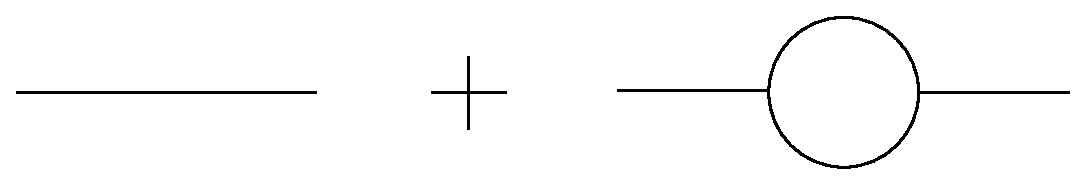
\includegraphics[width=0.8\textwidth]{./images/twoPointFunctionSelfEnergy}
  \caption{Self energy}
  \label{fig:twoPointFunctionSelfEnergy}
\end{figure}
To do so we need an expression for the free propagator of the $\phi$ field
\begin{equation}
  G_\phi = \frac{1}{p^2-M^2+i\epsilon}.
\end{equation}
Furthermore we need the result of the Feynman loop\-/diagram given in
\cref{fig:twoPointFunctionSelfEnergy}
\begin{equation}
  \Ima \mathcal{M}^{Loop} = \frac{\lambda^2}{32 \pi} \sqrt{1 - 4\frac{m^2}{M^2}} \theta(M - 2m)
\end{equation}
Summing over all possible self\-/energy graphs we get a geometric series
\begin{equation}
  i G(p^2) = \frac{i}{p^2 - m_R^2 + \Sigma(p^2) + i\epsilon },
\end{equation}
where we can plugin the free propagator and the result of the loop diagram of
our toy\-/Lagrangian to get a typical spectral function
\begin{equation}
  \begin{split}
    \rho(q^2) &= -\frac{1}{\pi} \Ima \Pi(q^2) \\
    &= \frac{1}{\pi} \Ima \left[ p^2 - M^2 + i\epsilon + \frac{\lambda^2}{32 \pi} \sqrt{1 - 4\frac{m^2}{M^2}} \theta(M - 2m) \right]^{-1} \\
    &= \delta(q^2 - M^2) + \theta(q^2 - 4m^2)\frac{\lambda^2}{32 \pi^2}
    \frac{1}{(q^2 - M^2)^2} \sqrt{\frac{q^2 - 4m^2}{q^2}},
  \end{split}
\end{equation}
where we have used \cref{eq:cuttingRules}.

  \end{document}